\documentclass{standalone}
\usepackage{tikz}
\usepackage{tabularx}
\usepackage{colortbl}
\usepackage{booktabs}
\usetikzlibrary{positioning}

\begin{document}
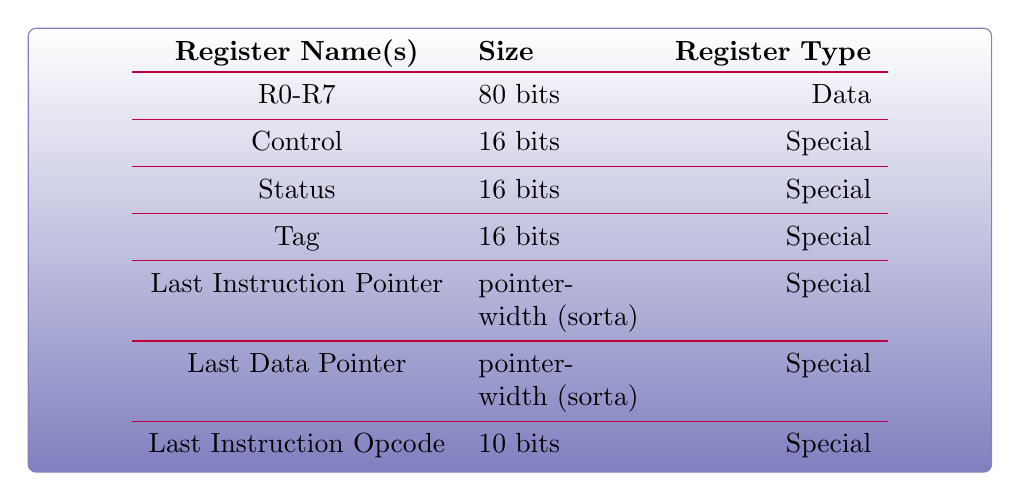
\begin{tikzpicture}[tab_style/.style={
	draw=blue!50!black!50,
	top color=white,
	bottom color=blue!50!black!50,
	rounded corners=1mm,
	text width=12cm,
	align=center
}]

\node[tab_style] (tbl) {
\begin{tabularx}{.8\textwidth}{cXrccc}
\arrayrulecolor{purple}
\textbf{Register Name(s)} & \textbf{Size} & \textbf{Register Type} \\
\toprule
R0-R7 & 80 bits & Data \\
\midrule
Control  & 16 bits & Special \\
\midrule
Status & 16 bits & Special \\
\midrule
Tag & 16 bits & Special \\
\midrule
Last Instruction Pointer & pointer-width (sorta) & Special \\
\midrule
Last Data Pointer & pointer-width (sorta) & Special \\
\midrule
Last Instruction Opcode & 10 bits & Special
\end{tabularx}
};

\end{tikzpicture}
\end{document}